\documentclass[a4paper, 12pt]{article}
\usepackage[left=2cm, text={17cm, 24cm}, right=2cm, top=2.5cm]{geometry}
\usepackage[czech]{babel}
\usepackage{times}
\usepackage[utf8]{inputenc}
\usepackage{graphics}
\usepackage{graphicx}
\usepackage{tabularx}
\usepackage{indentfirst}
\providecommand{\uv} [1] {\quotedblbase #1\textquotedblleft}
		
\begin{document}
\begin{titlepage}
\begin{center}
{\Huge \textsc{Vysoké učení technické v~Brně}\\ \huge \textsc{Fakulta informačních technologií\\}}
\vspace{\stretch{0.100}}
\includegraphics[width=135mm, height=40mm]{logo.png}\\
\vspace{\stretch{0.282}}
{\LARGE Databázové systémy\\2016/2017\\Konceptuální model\\ \Huge \textbf{Restaurace}}
\vspace{\stretch{0.618}}
\end{center}
{\Large Roman Nahálka (xnahal01) \hfill \today \\Martin Mihál(xmihal07)}
\end{titlepage}
\section{Zadání}
Vytvořte IS pro restaurační zařízení, který napomůže k~zjednodušení a~zpřehlednění jeho provozu. Restaurace je členěna do více místností a~má přední a~zadní zahrádku a~poskytuje běžné stravovací služby veřejnosti. Od informačního systému se požaduje, aby, krom jiného, umožnil správu rezervací a~objednávek. Rezervovat je možné jeden nebo více stolů v~místnostech či na zahrádkách, anebo celé místnosti, případně i~celou restauraci pro různé společenské akce. Součástí rezervace také může být objednávka nápojů a~jídel. Systém musí umožňovat zaměstnancům restaurace vkládat objednávky spolu s~informacemi, který zaměstnanec danou objednávku vložil a~pro koho je určena. Když se zákazníci rozhodnou zaplatit, musí jim systém vystavit účtenku. Po zaplacení pak příslušný zaměstnanec vloží záznam o~platbě do systému. Systém by měl také poskytovat podrobný přehled tržeb za vybrané období. Přístup k~této funkci bude mít pouze majitel. V neposlední řadě musí systém evidovat veškeré prodávané jídlo a~pití (včetně složení), přičemž majitel a~odpovědný vedoucí mají možnost měnit ceny jídla a~pití nebo přidávat a~odebírat položky.
\newpage
\section{Schéma databáze}
\begin{center}
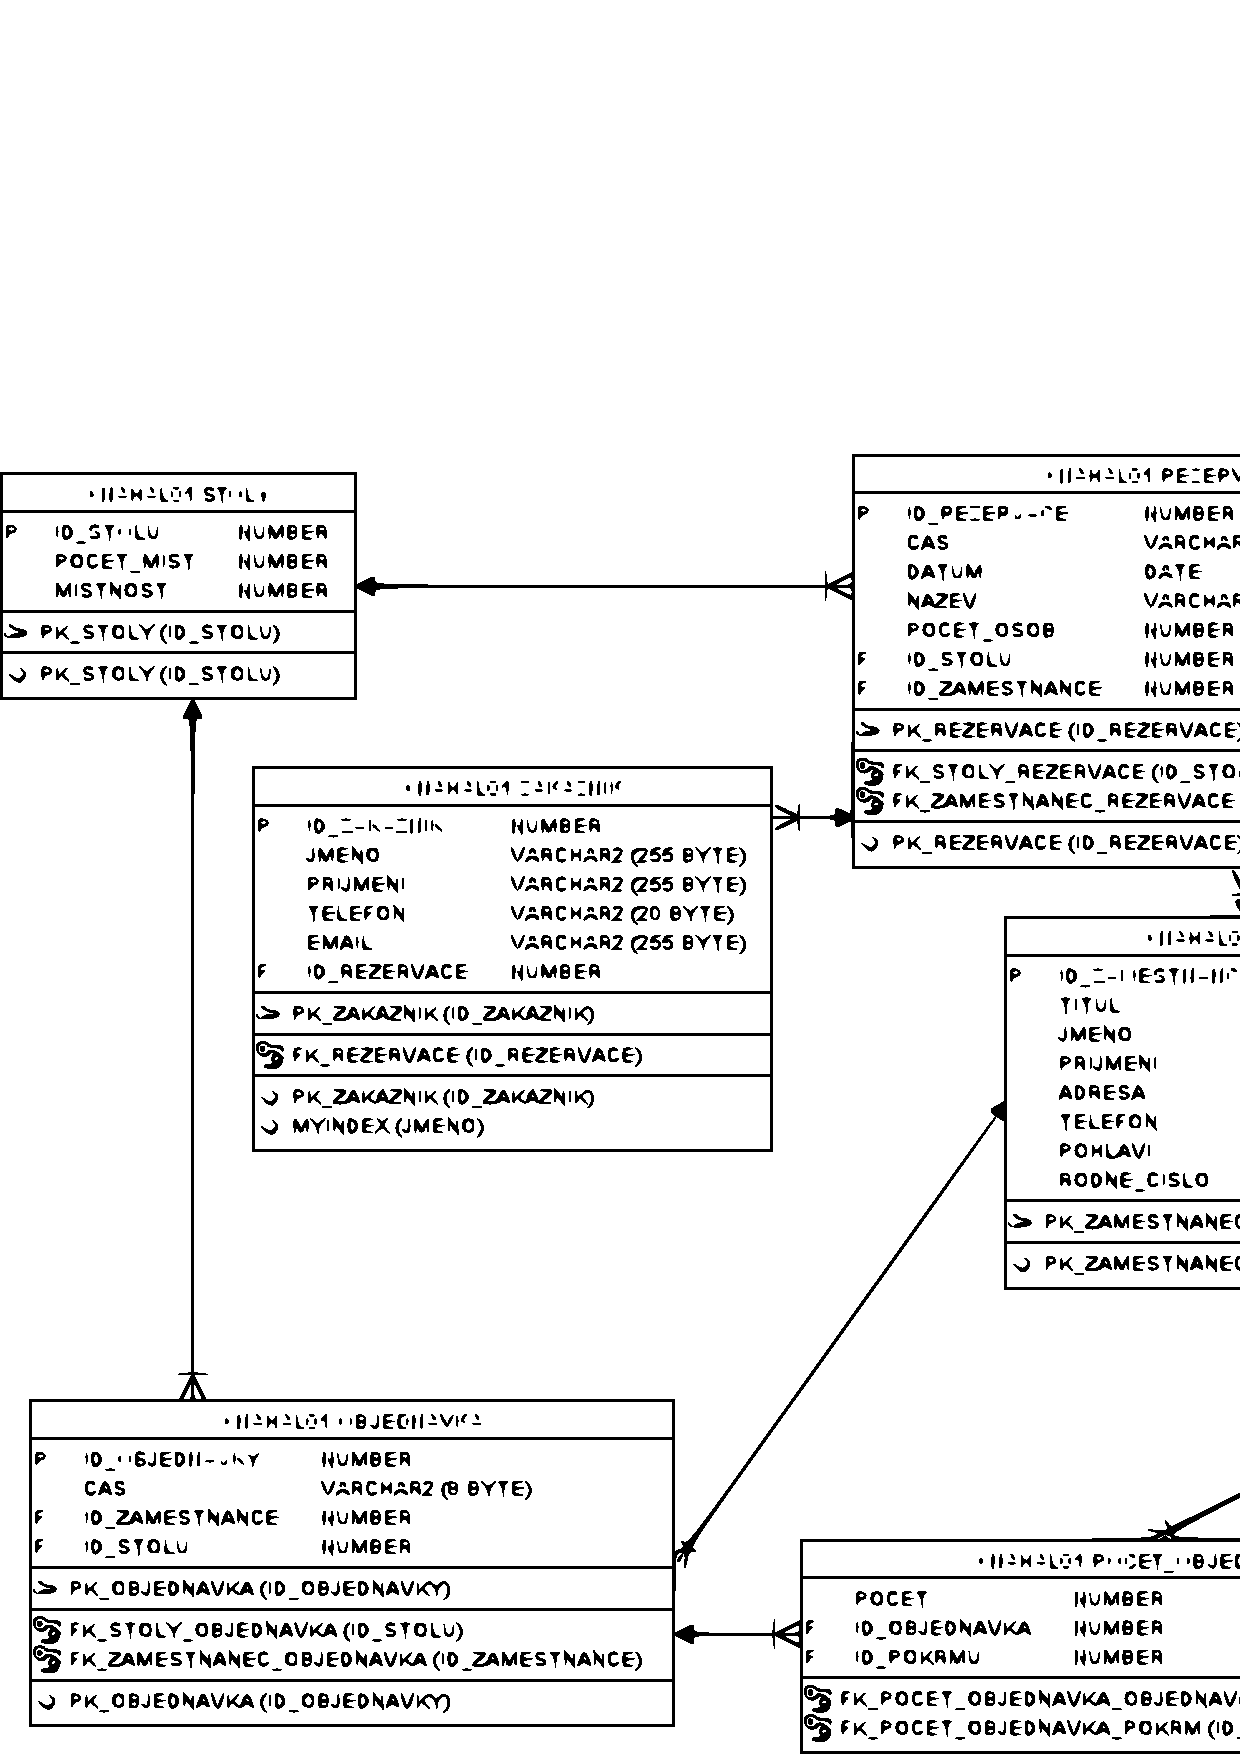
\includegraphics[width=190mm]{schema.png}
\end{center}
\newpage
\section{Implementace}
Byl navrhnut jednoduchý informační systém pro správu restaurací. Systém umožňuje evidenci objednávek, zaměstnanců, zákazníků, stolů, pokrmů a~surovin. Systém také umožňuje správu rezervací. K~těmto položkám mají právo zasahovat pouze zaměstnanci restaurace. 
\subsection{Triggery}
Skript obsahuje celkem tři triggery. V~prvních dvou případech se jedná o~automatickou inkrementaci primárního klíče, konkrétně v~tabulkách Rezervace a~Objednávka. Číslování těchto triggerů začíná na čísle 1. Třetím a~posledním triggerem je kontrola rodného čísla v~tabulce Zaměstnanec. Tento trigger při vložení nového zaměstnance do tabulky zkontroluje, že zadané rodné číslo zaměstnance je platné. Kontroluje tedy, že má platný rozsah 9--10 čísel a~zadané hodnoty pro rok, den a~měsíc narození jsou v~pořádku.
\subsection{Procedury}
Náš skript obsahuje celkem dvě procedury. První procedura je na výpis počet obsloužených zákazníku pro konkrétního zaměstnance. Druhá procedura vypíše počet rezervací, uskutečněných konkrétním zákazníkem.
\begin{itemize}
\item \verb|pocet_obslouzenych_zakaznikov| -- Procedura, která má jako vstupní parametr id zaměstnance ~ výstup je počet obsloužených lidí tímto zaměstnancem. V~případě neexistujícího zaměstnance je ošetřena výjimka.
\item \verb|pocet_rezervaci| -- Procedura, která má jako vstupní parametry jméno a~příjmení zákazníka a~výstup je počet rezervací provedených tímto zákazníkem. V~případě neexistujícího zákazníka je ošetřena výjimka.  
\end{itemize}
\subsection{Ukázkové výběry dat z~databáze}
Vytvořili jsme následující ukázky výběru dat z~databáze pro demonstraci funkčnosti databáze.
\begin{itemize}
\item Výpis objednávky, zaměstnance, který objednávku vytvořil a stolu.
\item Výpis typu pokrmu a počet pokrmů stejného typu.
\item Výpis zaměstnanců a počet objednávek, které mají přidělené.
\item Výpis zaměstnanců, kteří nemají přidělenou objednávku.
\item Výpis rezervací, kde je rezervovaný stůl s dvěma či více stoly.
\item Výpis jídla a jeho surovin.
\item Výpis zákazníků a jejich rezervací.
\end{itemize}
\subsection{Explain plan a vytvoření indexu}
Podle zadání jsme použili EXPLAIN PLAN pro výpis plánu provedení databázového dotazu. EXPLAIN PLAN jsme použili nad jednoduchým SELECTEM, který spojuje dvě tabulky, obsahuje agregační funkci a~používá klauzuli GROUP BY. Nejprve jsme spustili EPLAIN PLAN bez použití indexu a~poté s~indexem.
\begin{table}[h]
\small
\begin{tabular}{| r | l | c | r | c | r | c |}
\hline
Id & Operation & Name & Rows & Bytes & Cost(\% CPU) & Time\\
\hline
0 & SELECT STATEMENT &  & 3 & 504 & 4 (25) & 00:00:01\\
\hline
1 & HASH GROUP BY &  & 3 & 504 & 4 (25) & 00:00:01\\
\hline
2 & NESTED LOOPS & & 3 & 504 & 3 (0) & 00:00:01\\
\hline
3 & NESTED LOOPS & & 3 & 504 & 3 (0) & 00:00:01\\
\hline
4 & TABLE ACCESS FULL & ZAKAZNIK & 3 & 426 & 3 (0) & 00:00:01\\
\hline
* 5 & INDEX UNIQUE SCAN & PK\_REZERVACE & 1 & & 0 (0) & 00:00:01\\
\hline
6 & TABLE ACCESS BY INDEX ROWID & REZERVACE & 1 & 26 & 0 (0) & 00:00:01\\
\hline

\end{tabular}
\caption{EXPLAIN PLAN bez použití indexu}
\end{table}

\begin{table}[h]
\footnotesize
\begin{tabular}{| r | l | c | r | c | r | c |}
\hline
Id & Operation & Name & Rows & Bytes & Cost(\% CPU) & Time\\
\hline
0 & SELECT STATEMENT &  & 3 & 504 & 3 (34) & 00:00:01\\
\hline
1 & HASH GROUP BY &  & 3 & 504 & 3 (34) & 00:00:01\\
\hline
2 & NESTED LOOPS & & 3 & 504 & 2 (0) & 00:00:01\\
\hline
3 & NESTED LOOPS & & 3 & 504 & 2 (0) & 00:00:01\\
\hline
4 & TABLE ACCESS BY INDEX ROWID BATCHED & ZAKAZNIK & 3 & 426 & 2 (0) & 00:00:01\\
\hline
5 & INDEX FULL SCAN & MYINDEX & 3 & & 1 (0) & 00:00:01\\
\hline
* 6 & INDEX UNIQUE SCAN & PK\_REZERVACE & 1 & & 0 (0) & 00:00:01\\
\hline
7 & TABLE ACCESS BY INDEX ROWID & REZERVACE & 1 & 26 & 0 (0) & 00:00:01\\
\hline

\end{tabular}
\caption{EXPLAIN PLAN bez použití indexu}
\end{table}
Nejdříve jsme EXPLAIN PLAN zavolali bez použití námi vytvořeného indexu a~poté jsme EXPLAIN PLAN zavolali znovu s~použitím indexu. Jak můžeme vidět ve výše uvedených tabulkách, tak se snížila položka \texttt{Cost}, tedy počet zdrojů potřebných pro vykonání plánu, čím nižší je tato položka, tím efektivnější plán je. Naopak se nám zvýšilo vytížení CPU. Z~tabulky lze dále vyčíst, že při použití indexu se provede jedna operace navíc a~4. operace je nahrazena jinou. Rozebereme si jednotlivé operace v EXPLAIN PLAN:
\begin{itemize}
\item \texttt{SELECT STATEMENT} -- Znamená, že byl uskutečněný dotaz SELECT.
\item \texttt{HASH GROUP BY} -- Znamená, že se dotaz seskupí podle hashovacího klíče.
\item \texttt{NESTED LOOPS} -- Znamená, že spojované tabulky prohledává ve vnořených cyklech, tedy že se každý řádek první tabulky porovnává se všemi řádky druhé tabulky, atd.
\item \texttt{TABLE ACCESS FULL} -- Pouze u plánu bez indexu. Znamená, že se prochází celá tabulka od začátku bez použití indexů.
\item \texttt{TABLE ACCESS BY INDEX ROWID BATCHED} -- Pouze u plánu s indexem. Znamená, že se přistupuje do tabulky přes konkrétní řádek pomocí námi vytvořeného indexu.
\item \texttt{INDEX FULL SCAN} -- Pouze u plánu s indexem. Znamená, že provádí výpis hodnot z indexovaných sloupců.
\item \texttt{INDEX UNIQUE SCAN} -- Znamená, že se přistupuje k tabulkám přes B-strom, kdy nám vypadne jedinečný řádek podle primárního klíče, v tomto případě podle primárního klíče \texttt{PK\_REZERVACE}.
\item \texttt{TABLE ACCESS BY INDEX ROWID} -- Znamená, že se přistupuje do tabulky přes index.  
\end{itemize} 
\subsection{Přístupová práva}
V rámci projektu byli vytvořeny přístupová práva pro druhého člena týmu. Druhému členu týmu byl udělen přístup ke všem tabulkám a~procedurám databáze. 
\subsection{Materializovaný pohled}
Byl vytvořen materializovaný pohled patřící druhému členu týmu, který musel mít nastavené přístupové práva. Optimalizace pohledu proběhla pomocí logů. Díky tomu se nemusí celá tabulka obnovovat, ale zachytávají se jenom změny a~ty se aktualizují. Následně byl vytvořen pohled. Použili jsme následující způsoby optimalizace:
\begin{itemize}
\item \texttt{CACHE} -- Využije se cache paměť pro rychlejší načtení dat.
\item \texttt{BUILD IMMEDIATE} -- Hned po vytvoření se pohled naplní daty.
\item \texttt{REFRESH FAST ON COMMIT} -- Rychlá aplikace změn.
\item \texttt{ENABLE QUERY REWRITE} -- Použitelnost pohledu pro optimalizátor.
\end{itemize}                        
                                                                                                                                                                                    
\end{document}
